\section{User interface design}
In this section are presented some mockups of the main features and related user interfaces the system is supposed to offer to the user and to the customer care through the proper web-based application.
\subsection{User app}
The user app must have a charming and intuitive user interface in order to provide a easy-to-use experience to the user. That interface must be optimized for mobile devices even if the application is accessible and must be usable from every web browser on different size devices.

\subsubsection{Login page}
Simple initial page for the application to allow the user to authenticate to the system through username and password. A new user can access the registration process through the \emph{New User} button. \\
As specified in the requirements section, that page also allows a guest user or a \emph{banned} registered user to access to customer care contact information through the \emph{Contact us} button. \\
If a user is not recognized or is banned an error alert is shown when credential are submitted.

	\begin{figure}[h]
			\centering
			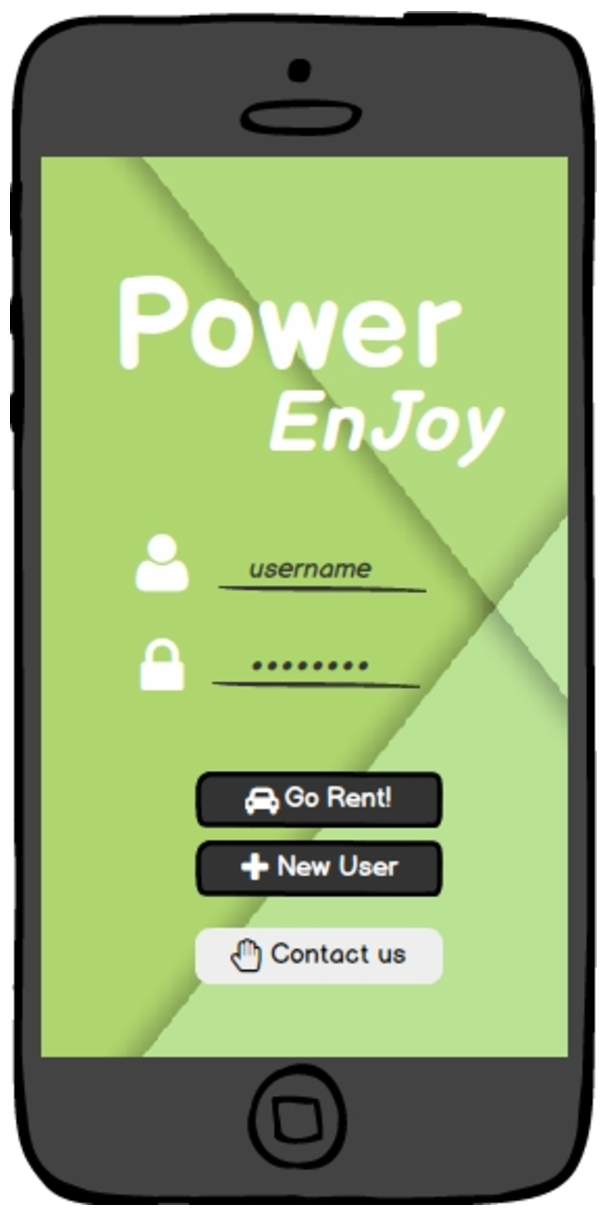
\includegraphics[width=0.4\linewidth]{mockups/loginPage}
			\caption{
				\label{fig:loginPage} 
				Login page
			}
		\end{figure}
		

\subsubsection{Home page}
The home page shows to a logged user all the possible functionalities provided from the app:
\begin{itemize}
	\item See available cars and reserve one of them (eventually with the \emph{Money Saving Option})
	\item Unlock a car (disabled button in the mockups, it would be active only if there is an active reservation for the registered user logged in)
	\item See user's information and edit them
	\item See user's rent history
	\item See user's payment history
	\item Show customer care contact information
\end{itemize}

That page shows also the user's name to ensure to the user he has been correctly recognized by the system and to make the interface more customized. \\

The icon in the right corner, from that page, brings the user to the functionality of see available cars; on all other pages (without the orange position icon) it brings the user to that page: the home page.

	\begin{figure}[h]
			\centering
			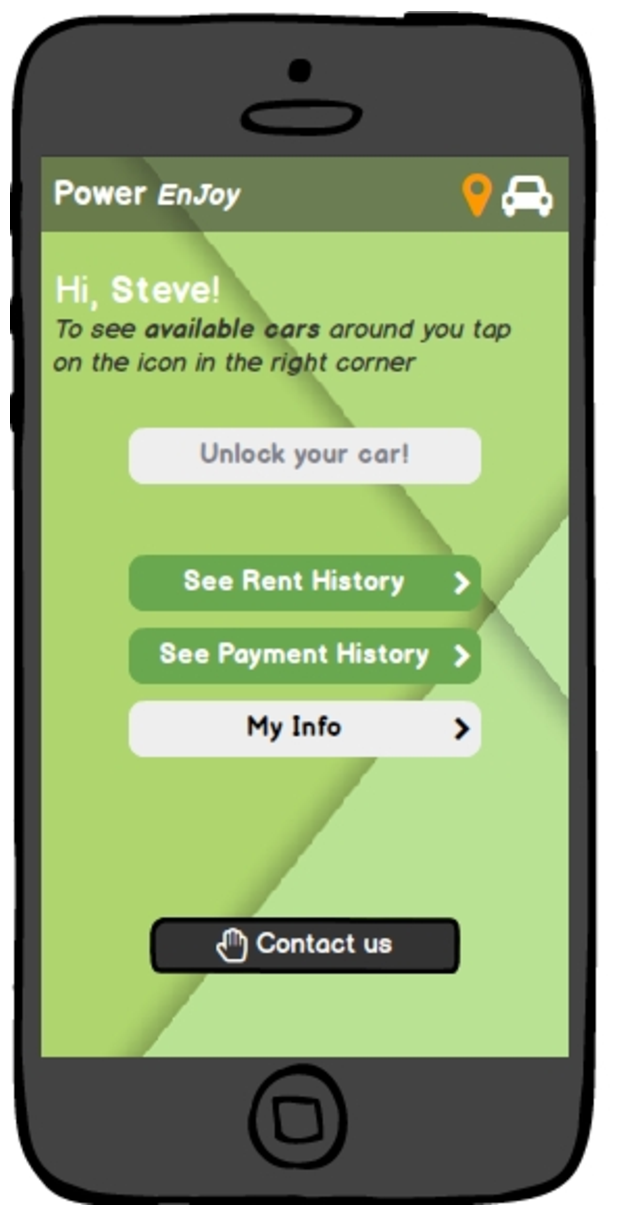
\includegraphics[width=0.4\linewidth]{mockups/homePage}
			\caption{
				\label{fig:homePage} 
				Home page
			}
		\end{figure}


\subsection{Customer care app}